\documentclass[13pt, letterpaper, twoside]{book}
\usepackage{graphicx}

\usepackage[driver=xetex,paperwidth=8.5in,paperheight=11in,left=1.1in, right=1.74in,top=1.4in, bottom=1.74in]{geometry}
\usepackage[no-math]{fontspec}

\usepackage{sectsty, tikz, color}
\usepackage{multicol}
\usepackage{amsmath, amssymb, amsfonts,  titlesec}
\usepackage[urw-garamond]{mathdesign}
\usepackage{fancyhdr, booktabs}
%\usepackage[font=small,format=plain,labelfont=it,textfont=it]{caption}
\usepackage{caption,subcaption}
\usepackage{listings}
% \usepackage[T1]{fontenc} 
\usepackage{enumitem}

 \DeclareTextCommandDefault{\nobreakspace}{\leavevmode\nobreak\ } 

%========== DEFINITIONS ==========

\newlist{alist}{itemize}{1}
\setlist[alist]{label=--,labelindent=2in,leftmargin=9pt,labelsep=6pt, itemsep=0pt}

\def\Lmax{L_{\text{max}}}

%========= FONT SPECS ============
\tolerance 8000

\defaultfontfeatures{Mapping=tex-text, Ligatures=Common}

%\renewcommand\refname{references} % this sets the name of
\def\labelitemi{--}

\def\sansfont{\fontspec[Script=Latin,LetterSpace=2.6, Mapping=tex-text]{DIN 1451 Mittelschrift}}
\def\sansitalicfont{\fontspec[Script=Latin,LetterSpace=2.6, FakeSlant=0.2, Mapping=tex-text]{DIN 1451 Mittelschrift}}

\def\monofont{\fontspec[Script=Latin,Mapping=tex-text,Scale=0.91, AutoFakeBold]{Inconsolata}}

\renewcommand{\texttt}[1]{{\monofont #1}}

%========== COLOR STUFF ===============

\definecolor{darkred}{rgb}{0.6, 0, 0.00}


%============ LISTINGS ==============
\lstset{
aboveskip=2\medskipamount, belowskip=2\medskipamount,
basicstyle=\monofont,
language=python,
numbers=left, numberstyle=\tiny,  numbersep=9pt,
xleftmargin=.4in, frame=l, xrightmargin=1.74in
}


%============= PAGE LAYOUT ============

%\titleformat{\section}{\huge\sansnormalfont}{\protect\makebox[0pt][r]{\thesection\quad}}{0em}{}
\titleformat{\chapter}{\fontsize{32pt}{36pt}\selectfont\sansfont}{}{0em}{}
\titleformat{\section}{\fontsize{18pt}{22pt}\selectfont\sansfont}{\protect\makebox[0pt][r]{\thesection\quad}}{0em}{}
\titleformat{\subsection}{\fontsize{12pt}{16pt}\selectfont\sansfont}{\protect\makebox[0pt][r]{\thesubsection\fontsize{18pt}{22pt}\selectfont\quad}}{0em}{}
%\titleformat{\paragraph}{\fontsize{12pt}{16pt}\selectfont}{}{}{}

\fancyhead[LE]{\sansfont\small An improved batch CP method \normalsize}
\fancyhead[RE]{}
\fancyhead[LO]{}
\fancyhead[RO]{\sansfont\small \nouppercase\rightmark}
\fancyfoot[C]{\sansfont\thepage}

\fancypagestyle{plain}{
\fancyhf{}
\renewcommand{\headrulewidth}{0pt}
\fancyfoot[C]{\sansfont\thepage}
}



\begin{document}
\frontmatter

\fontsize{12pt}{16pt}\selectfont
\thispagestyle{empty}
\pagestyle{fancy}

\baselineskip=16.8pt plus 0pt
\frenchspacing

\begin{centering}
\vspace{3em}
\LARGE\sansfont{Scheduling non-identical jobs on a batch resource\\-- Interim
Report --}

\vspace{2em}
\large
\sansfont Sebastian Kosch\\
997 241 024

\vfill
\normalfont
\fontsize{12pt}{16pt}\selectfont
A thesis submitted in conformity with the requirements

for the degree of \textit{Bachelor of Applied Science}

\vspace{1em}
Supervisor: Prof. J. Christopher Beck, MIE

\vspace{2em}

\textmd Division of Engineering Science\\
University of Toronto\\

2013

\end{centering}
\pagebreak

%\include{firstpage}

\tableofcontents

\mainmatter
\pagebreak
\vskip 4em
\chapter{Introduction}

\chapter{Fundamentals}
Some introductory paragraphs on minimization/maximization problems.
\section{Linear programming models}
An introduction to and illustration of LP models.
\subsection{Problem motivation}
\subsection{Graphical explanation}
\section{Integer programming models}
An introduction to and illustration of MIP models
\subsection{Solution technique}
\subsection{Other methods}
\section{Constraint programming models}
\subsection{Concept}
\subsection{Solution}
\subsection{Global constraints}

\chapter{Problem description}
\section{Characteristics of the problem}
\section{Summary of Malapert's approach}
In MIP terms, Malapert's approach was to minimize $\Lmax$ subject to the following constraints:

\begin{alignat}{2}
  &\sum_{k \in K} x_{jk} = 1 \quad && \forall j \in J \\
  &\sum_{j \in J} s_j x_{jk} \leq b \quad && \forall k \in K\\
  &p_j x_{jk} \leq P_k \quad && \forall j \in J, \forall k \in K\\
  &C_{k-1} + P_{k} = C_k \quad && \forall k \in K\\
  &(d_{max} - d_j)(1 - x_{jk}) + d_j \geq D_k \quad && \forall j \in J, \forall k \in K\\
  &D_{k-1} \leq D_k \quad && \forall k \in K \label{malapp-edd} \\
  &C_k - D_k \leq \Lmax \quad && \forall k \in K\\[2ex]
  &C_k \geq 0, P_k \geq 0 \text{ and } D_k \geq 0 \quad && \forall k \in K  
\end{alignat}

The constraint \ref{malapp-edd} is the EDD constraint.

\section{Improved bounds in MIP}

\subsection{Lower bound on {\sansitalicfont L}\textsubscript{max}}

A lower bound on $\Lmax$ can be found using the completion date of the fully elastic cumulative solution and comparing it with the latest due date:
\begin{align}
& \Lmax \geq \frac{1}{b} \sum_{j \in J} s_j p_j - \mathrm{max}(d_j) \label{eq:lmaxlb}
\end{align}
The right hand side involves no decision variables and can be computed in $O(n_j)$ beforehand. This is a valid lower bound: no batch configuration will ever achieve a tighter packing than a fully elastic solution. Even if, in the elastic case, the job with the last due date is scheduled last, it will have a lateness $L_{\text{last}}$ equal to the term in \ref{eq:lmaxlb}. Any other scheduling in the elastic case will result in a worse $L_{\text{last}}$. Since $\Lmax \geq L_{\text{last}}$, this is a lower bound.

In fact, we can go one step further and calculate this lower bound $L_{\text{last}}$ for all sorted subsets $M$ of $J$. First, sort all jobs by non-decreasing due date. This can be done in $O(n_j \log n_j)$. Then the subset $M_1$ contains the job with the earliest due date, $M_2$ contains $M_1$ as well as the next job, etc. until $M_{n_j}$ contains all jobs. The above consideration is certainly true for every subset $M$ containing $m$ jobs.

The reasoning is analogous to that behind the EDD rule. Suppose we assigned a job with a later-than-earliest due date first, then $L_{\text{last},M_1}$ would be reduced; however the earliest-due job would then have to be scheduled at a later point, say in $M_5$: this would increase $L_{\text{last},M_5}$ by an amount not less than was saved by $L_{\text{last},M_1}$. Since we need the lowest possible value for $L_{\text{last}}$ to be certain of its validity as a lower bound, that would be unacceptable. The constraints are thus:
\begin{alignat}{2}
& \Lmax \geq \frac{1}{b} \sum_{j_1 \in J}^{j_m \in J} s_j p_j - d_m \quad && \forall m \in \{1, \dots, n_j\}
\end{alignat}
and require prior sorting of jobs by due dates.

\subsection{Upper bound on {\sansitalicfont L}\textsubscript{max}}
An upper bound on $\Lmax$ can be found by using a dispatch rule to find a feasible, if not optimal, schedule. I present several dispatch rules:

\paragraph{\fontsize{12pt}{14pt}\selectfont Earliest due date first} This is a basic one: The given formulation lacks a rule that ensures that no empty batch is followed by a non-empty batch. Empty batches have no processing time and a due date only bounded by $d_\text{max}$, so they can be sequenced between non-empty batches without negatively affecting $\Lmax$. Since, however, desirable schedules have no empty batches

\subsection{No postponing of jobs to later batches}
Since the jobs are already sorted by non-decreasing due dates, it makes sense to explicitly instruct the solver never to attempt to push jobs into batches with a greater index than their own: even if every job had its own batch, it would be unreasonable to ever postpone a job to a later batch.
\begin{alignat}{2}
  & x_{jk} = 0 \quad && \forall j,k : j > k
\end{alignat}

\subsection{Grouping empty batches}
The given formulation lacks a rule that ensures that no empty batch is followed by a non-empty batch. Empty batches have no processing time and a due date only bounded by $d_\text{max}$, so they can be sequenced between non-empty batches without negatively affecting $\Lmax$. Since, however, desirable schedules have no empty batches scattered throughout, we can easily reduce the search space by disallowing such arrangements. The idea is illustrated in Figure \ref{fig:dominancerule}.


\begin{figure}
  \centering
  \begin{subfigure}[b]{0.4\textwidth}
    \centering
    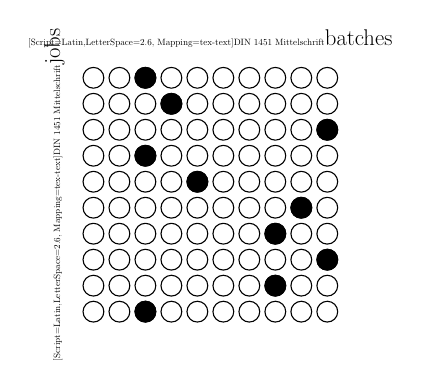
\begin{tikzpicture}[scale=0.33]
      \pgftext[x=-1.5cm, y=4.5cm, rotate=90]{\sansfont\Huge jobs}
      \pgftext[x=4.5cm, y=10.5cm]{\sansfont\Huge batches}

      \foreach \j in {0,...,9}
      {
        \foreach \k in {0,...,9}
        {
          \draw[] (\k, \j) circle [radius=0.4];
        }
      }
      \draw [fill] (2,0) circle [radius=0.4];
      \draw [fill] (2,6) circle [radius=0.4];
      \draw [fill] (2,9) circle [radius=0.4];
      \draw [fill] (3,8) circle [radius=0.4];
      \draw [fill] (4,5) circle [radius=0.4];
      \draw [fill] (7,1) circle [radius=0.4];
      \draw [fill] (7,3) circle [radius=0.4];
      \draw [fill] (8,4) circle [radius=0.4];
      \draw [fill] (9,2) circle [radius=0.4];
      \draw [fill] (9,7) circle [radius=0.4];
    \end{tikzpicture}
    \caption{Without dominance rule}
  \end{subfigure}
  \begin{subfigure}[b]{0.4\textwidth}
    \centering
    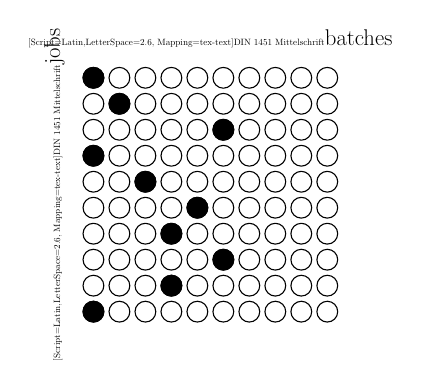
\begin{tikzpicture}[scale=0.33]
      \pgftext[x=-1.5cm, y=4.5cm, rotate=90]{\sansfont\Huge jobs}
      \pgftext[x=4.5cm, y=10.5cm]{\sansfont\Huge batches}

      \foreach \j in {0,...,9}
      {
        \foreach \k in {0,...,9}
        {
          \draw[] (\k, \j) circle [radius=0.4];
        }
      }
      \draw [fill] (0,0) circle [radius=0.4];
      \draw [fill] (0,6) circle [radius=0.4];
      \draw [fill] (0,9) circle [radius=0.4];
      \draw [fill] (1,8) circle [radius=0.4];
      \draw [fill] (2,5) circle [radius=0.4];
      \draw [fill] (3,1) circle [radius=0.4];
      \draw [fill] (3,3) circle [radius=0.4];
      \draw [fill] (4,4) circle [radius=0.4];
      \draw [fill] (5,2) circle [radius=0.4];
      \draw [fill] (5,7) circle [radius=0.4];
    \end{tikzpicture}
    \caption{With dominance rule}
  \end{subfigure}
\caption{Dominance rule to eliminate empty batches followed by non-empty batches
(circles represent the $x_{jk}$ variables; a filled circle stands for $x_{jk} =
1$)}\label{fig:dominancerule}
\end{figure}


A mathematical formulation is
\begin{alignat}{2}
& \sum_{j \in J} x_{j,k-1} = 0 \rightarrow \sum_{j \in J} x_{jk} = 0 \quad && \forall k \in K. \label{eq:emptybatch0}
\end{alignat}

To implement this, we can write constraints in terms of an additional  set of binary variables, $e_k$, indicating whether a batch $k$ is empty or not:

\begin{alignat}{2}
& e_k + \sum_{j \in J} x_{jk} \geq 1 \quad && \forall k \in K, \label{eq:emptybatch1} \\
& n_j (e_k-1) + \sum_{j \in J} x_{jk} \leq 0 \quad && \forall k \in K. \label{eq:emptybatch2}
\end{alignat}

Constraint \ref{eq:emptybatch1} enforces $e_k = 1$ when the batch $k$ is empty. Constraint \ref{eq:emptybatch2} enforces $e_k = 0$ otherwise, since the sum term will never exceed $n_j$. The rule \ref{eq:emptybatch0} can now be expressed as $e_{k-1} = 1 \rightarrow e_k = 1$, and implemented as follows:

\begin{alignat}{2}
& e_k - e_{k-1} \geq 0 \quad && \forall k \in K.
\end{alignat}

We can also prune any attempts to leave the first batch empty by adding a constraint $e_0 = 0$.

{\color{darkred} This, while it works just fine, actually takes longer than without it.}

\subsection{Bounding the number of batches \sansitalicfont n\textsuperscript{k}}
Initially, the number of batches needed is assumed to be equal to the number of jobs: $n_k = n_j$. Reducing $n_k$ by pre-computing the maximum number of batches needed shrinks the $x_{jk}$ matrix.

Unfortunately, we cannot make a general statement that optimal solutions never have more batches than other feasible solutions -- a simple counterexample is shown in figure \ref{fig:bnk1}.\footnote{To be more precise, we cannot state that at least one optimal solution is in the subset of feasible solutions that uses the fewest number of batches -- a dominance situation that could be exploited, were it true.}


\begin{figure}
  \centering
  \begin{subfigure}[b]{0.4\textwidth}
    \centering
    \begin{tikzpicture}[scale=0.2, font=\scriptsize]

      \draw [<->,thick] (0,12) node (yaxis) [above] {\sansitalicfont s}
        |- (25,0) node (xaxis) [right] {\sansitalicfont t};
      \draw[dotted] (0,10) -- (25,10);
        \draw (0,0) rectangle (5,7) node[fn] {$p = 10$\\$d = 10$\\$L = 0$};
        \draw (5,0) rectangle (20, 3) node[fn] {$p = 30, d=20, L=10$};
        
    \end{tikzpicture}
  \end{subfigure}
  \begin{subfigure}[b]{0.4\textwidth}
    \centering
    \begin{tikzpicture}[scale=0.2, font=\scriptsize]

      \draw [<->,thick] (0,12) node (yaxis) [above] {\sansitalicfont s}
        |- (25,0) node (xaxis) [right] {\sansitalicfont t};
      \draw[dotted] (0,10) -- (25,10);
        \draw (0,0) rectangle (5,7) node[fn] {$p = 10$\\$d = 10$\\$L = 20$};
        \draw (0,7) rectangle (15, 10) node[fn] {$p = 30, d=20, L=0$};
    
    \end{tikzpicture}
  \end{subfigure}
\caption{Overzealous batch elimination can increase $\Lmax$}\label{fig:bnk1}
\end{figure}

It is perhaps possible, however, to generate a feasible solution that is likely to use $n_k < n_j$ and to guarantee that such a solution will never use fewer batches than the optimal solution. To do this, let the initial solution $\pi_0$ be a schedule in which every job is assigned to one batch (i.e. $n_k = n_j$) and the jobs are ordered by non-decreasing due date (i.e. $d_n \leq d_{n+1}$), as in figure \ref{fig:bnk2}.

%\input{figure showing all the jobs in EDD sequence}




Capacity permitting, jobs are now moved into earlier batches to improve the schedule, eliminating the batch they were placed in initially. Every such move reduces $n_k$ by one.

 Two types of moves are possible: \textit{safe} moves and \textit{risky} moves. A move is safe when a job is moved into an earlier batch of longer processing time. A move is risky when a job is moved into an earlier batch of shorter processing time, thus increasing the lateness of that batch.

Moving a job has three effects: 

\begin{alist}
\item{Effect on the batches after}
\item{Effect on the batches between, including the new job}
\item{Effect on the job itself}
\end{alist}

\begin{table}
\centering
\begin{tabular}{r c c}
\toprule
              & safe                 & risky \\
\midrule
batches after & lateness improves by $p_j$ & lateness improves by $p_a$ \\
batches between & --- & lateness worsens by $p_j - p_a$ \\
job itself & lateness improves & lateness improves\\ 
\bottomrule
\end{tabular}
\caption{Lateness effects of safe and risky moves}
\end{table}

We can easily generate a solution that only contains safe moves.
We now need to prove that our relaxed solution $\pi_{\text{edd}}$ will never use fewer batches than the optimal solution $\pi_{\text{opt}}$.

For this to be true, we need to show that if there is ever a situation in which we could \textit{either} make $n$ unsafe moves \textit{or} $m>n$ safe ones, using the unsafe ones will never be beneficial if the remaining $m-n$ safe candidates cannot be moved somewhere else.

We're trying to find a relaxation of the problem that is guaranteed to generate as least as many batches as the optimal solution.


Whenever there is an alternative between $n$ unsafe moves and $>n$ safe ones, perform $n$ safe ones. Whenever only an unsafe is available, eliminate none and proceed to the next batch.

Unfortunately, we cannot generally state that optimal solutions never have more batches than other feasible solutions: when a job $j_b$ is moved into a prior batch holding $j_a$ and $d_b > d_a$ as well as $p_a < p_b$, it can sometimes happen that $\Lmax$ is increased.

\subsubsection{Some stuff to try}

We can try only considering jobs \textit{before} $\Lmax$, because anything after that job wouldn't be moved in an optimal solution. 

\begin{alist}
\item {Never move a job into a batch with greater lateness than itself. This would never improve $\Lmax$ and is therefore a dangerous elimination.}
\item {
\end{alist}
  

We can, however, use a dispatch rule to get an upper bound on the number of batches used.

Does the optimal schedule always ever have more batches than a non-optimal schedule? 


\section{Known constraints, unused}
Anything that comes \textit{after} $\Lmax$ doesn't matter. If $L$ is decreasing after $\Lmax$, the jobs must not be stacked ever.




\section{Constraint Programming model}
The same problem can be formulated as a basic constraint programming model without global constraints: 
\begin{alignat}{2}
 &\sum_{k \in K} x_{jk} = 1 \quad && \forall j \in J \\
  &\sum_{j \in J} s_j x_{jk} \leq b \quad && \forall k \in K\\
  &P_k = \max(p_j x_{jk}) \quad && \forall k \in K\\
  &C_{k-1} + P_{k} = C_k \quad && \forall k \in K\\
  &D_k = \min(d_j x_{jk}) \quad && \forall k \in K\\
  &D_{k-1} \leq D_k \quad && \forall k \in K \label{malapp-edd} \\
  &\Lmax = \max(C_k - D_k) \quad && \forall k \in K\\[2ex]
  &C_k \geq 0, P_k \geq 0 \text{ and } D_k \geq 0 \quad && \forall k \in K  
\end{alignat}

Batches are interval variables who have start and end times and precedence constraints of the type \texttt{IloEndAtStart(env, batch1, batch2, 0)}. 

\section{Test data for evaluation}
Malapert uses benchmark data by Daste. For design purposes, I created my own set of randomized job lists, with $s_j, p_j \in [1, 20]$ and $d_j \in [1, 10n]$ where $n$ is the number of jobs. Here is the Python code used:

\lstset{language=Python}
\begin{lstlisting}
import csv
import random

random.seed(None)

for i in range(10,100,20):
    with open( "data_" + str(i), "wb") as csvfile:
        csvwriter = csv.writer(csvfile, delimiter=",")
        csvwriter.writerow(['s_j', 'p_j', 'd_j'])
        for job in range(i):
            csvwriter.writerow([random.randrange(1,20),
               random.randrange(1,20),
               random.randrange(1,5*i)])
    csvfile.close()
\end{lstlisting}

CSV files can be read in with \texttt{IloCsvReader} and \texttt{IloCsvLine}.


\chapter{My solution}
\section{MIP formulation improvements}
\section{CP formulation improvements}

\chapter{Discussion}


\pagebreak

\vskip 4em
\section[Intro]{Introduction}
\vspace{6.6em}

Books to read: Model Building in Mathematical Programming by HP Williams

Mathematical programming models all involve optimization. They want to minimize or maximize some objective function.

There are linear programming models, non-linear programming models and integer programming models.

Constraint programming and Integer Programming are twins and can usually be translated into one another. In CP each variable has a finite domain of possible values. Constraints connect/restrict the possible combinations of values which the variables cantake. These constraints are of a richer variety then the linear constraints of IP and are usually expressed in the form of predicates, such as ``all\_different(x1, x2, x3)''. The same condition could be imposed via IP, but it's more troublesome to formulate. Once one of the variables has been set to one of the values in its domain (either temporarily or permanently), this predicate would imply that this value must be taken out of the domain of all other variables (``propagation''). In this way constraint propagation is used until a feasible set of values is found (or not).

CP is useful where a problem function has no objective function and we are just looking for a feasible solution. We can't prove optimality, although we could using IP.

Comparisons and connectionsbetween IP and CLP are discussed by Barth (1995), Bockmayr and Kasper (1998), Brailsford
et al.
(1996), Prolland Smith (1998), Darby-Dowman and Little (1998), Hooker (1998) and Wilson and Williams (1998). Theformulation of the all\_different predicate using IP is discussed by Williams and Yan (1999).

The first approach to solving a multi-objective problem is to solve the model a number of times with each objective function in turn. The result may give an idea of what to do next.


\subsection{Chapter 8: Integer Programming}

The real power of IP as a method of modelling is that of binary constraints, where variables can take on values of 0 or 1. Maybe it should be called ``discrete programming.'' Precise definitions of those problems that can be formulated by IP models are given by Meyer (1975) and Jeroslow (1987). 

Problems with discrete inputs and outputs are the most obvious candidates for IP modelling (``lumpy inputs and outputs''). Sometimes solving an LP and rounding to the nearest integer works well, but sometimes it doesn't, as demonstrated in Williams, first example in 8.2. The smaller the variables (say, <5), the greater significance those rounding problems will have. 

When input variables have small domains, say, machine capacities, then again this may rule out LP relaxations. A good example of an IP problem is the knapsack assignment problem. A single constraint is that the capacity of the knapsack cannot be exceeded. Any LP formulation would always fill the knapsack 100\%, ignoring the discrete size of the objects. Two other well-known types of problems include \textit{set partitioning problems} and \textit{aircrew scheduling problems}. 

Integer programming models cannot be solved directly, but need to be brute-forced in a tree search manner. The search space, however, can be greatly reduced by a number of bounding techniques often depending on the nature of the problem. That is why the general method of IP solving is called \textit{branch-and-bound}.

So-called \textit{cutting planes methods} usually start by solving an IP problem as LP. If the resulting solution is integral, we're happy. Otherwise extra constraints (cutting planes) are added to the problem, further constraining it until an integer solution is found (or, if none can be found, we're out of luck). Cutting planes make for nice illustrations they are not very efficient with large problems. Cutting planes were invented by Gomory (1958).

Enumerative methods are generally applied to pure binary problems, where the search tree is pruned. The best known of these methods is Balas's additive algorithm described by Balas (1965). Other methods are givenby Geoffrion (1969). A good overall exposition is given in Chapter 4 of Garfinkel and Nemhauser (1972).

There are so-called \textit{pseudo-boolean methods} to solve pure binary problems that take boolean constraints as inputs. That may be comfortable for the user sometimes, but is rarely used in practice.

Generally, branch-and-bound methods first solve the LP relaxation to check whether we're lucky enough to find an integer solution. If not, a tree search is performed. 

\subsection{Chapter 9: Building IP models I.}

Binary variables are often called 01-variables. Decision variables could also have a domain like $\{0,1,2\}$ or $\{4,12,102\}$. Decision variables, especially the 01 kind, can be linked to the state of continuous variables like this: $x-M\delta \leq 0 \leftrightarrow x>0 \rightarrow \delta = 1$, where we know that $x < M$ is always true.

To use a 01 variable to indicate whether the following is satisfied:
\begin{align}
2x_1 + 3x_2 &\leq 1\\
x_1 &\leq 1\\
x_2 &\leq 1,
\end{align}
so, mathematically speaking,
\begin{align}
\delta = 1 &\rightarrow 2x_1 + 3x_2 \leq 1\\
2x_1 + 3x_2 \leq 1 &\rightarrow \delta = 1,
\end{align}
Then we can argue that at most, $2x_1 + 3x_2 = 5$, so
\[
2x_1 + 3x_2 + 4\delta \leq 5
\]
will ensure that $\delta = 1$ forces the equation to be true: use $M = 2 + 3 - 1$ to find $4$. In order to enforce $\delta = 1$ if the equation is true, use $m = 0 + 0 -1$ and write
\[
2x_1 + 3x_2 + \delta \geq 1
\]

All kinds of logical conditions can be modelled using 01 variables, although it's not always obvious how to capture them in that format. 

Logical conditions are sometimes expressed within a Constraint Logic Programming language as discussed inSection 2.4. The tightest way of expressing certain examples using linear programming constraints is described byHooker and Yan (1999) and Williams and Yan (1999). There is a close relationship between logic and 01 integerprogramming, which is explained in Williams (1995), Williams and Brailsford (1999) and Chandru and Hooker(1999).

\paragraph*{Special Ordered Sets}
Two very common types of restriction arise in mathematical programming, so two concepts (SOS1 and SOS2) have been developed. An SOS1 is a set of variables within which exactly one variable must be non-zero and the rest zero. An SOS2 is a set where at most two can be non-zero, and the two variables must be adjacent in the input ordering. Using a branch-and-bound algorithm specialized for SOS1 or SOS2 sets can speed things up greatly.

\paragraph*{Disjunctive constraints}
It is possible to define a set of constraints and postulate that at least one of them be satisfied.

\subsection{Special kinds of IP models}
Most practical IP models do not all into any of these categories but arise as MIP models often extending an existing LP model. Here are some examples.

\paragraph*{Set covering problems} We have a set $S = \{1,2,3,\dots,m\}$. We have a bunch of subsets $\mathcal{S}$ of subsets, each associated with a cost. Now cover all members of $S$ using the least-cost members of $\mathcal{S}$.

\paragraph*{Knapsack problem} These are the really simple ones with just one constraint, namely the constraint of not being able to take more items with you than the knapsack can carry while maximizing the value of the taken objects.

\paragraph*{Quadratic assignment problem} Two sets of objects $S$ and $T$ of the same size require the objects to be matched pairwise. There are costs associated with pairs of pairs, that is the cost $c_{ij,kl}$ is the cost of assigning $i$ to $j$ while also assigning $k$ to $l$. This cost will be incurred if both $\delta_{ij}$ and $\delta_{kl}$ are \texttt{true}, i.e. $\delta_{ij}\delta_{kl} = 1$. The objective function is a quadratic expression in 01 variables:
\begin{align}
\mathrm{Minimize}\;\sum^n_{\substack{i,j,k,l=1\\k>l}} c_{ij,kl}\delta_{ij}\delta_{kl}
\end{align}
The quadratic version is practically unsolveable, so to be able to enumerate the possible assignments the above objective function has to be split up into separate constraints, which obviously means there will be an explosion in problem size as the number of variables grow.

\subsection{How to formulate a good model}
According to Williams, it is easy to build IP models that, while correct, are really inefficient. Fortunately, with some knowledge of what happens behind the scenes (and some practice), sucky models can often be improved. One good method to know (although it doesn't help by itself) is to turn a general integer variable into a bunch of 01 variables. Say $\gamma$ is a general, non-negative integer variable with a known upper bound of $u$, then we can replace it with $\delta_0 + 2\delta_1 + 4\delta_2 + 8\delta_3 + \dots + 2^n\delta_n$. 

\paragraph*{Example problem} 
http://www.scribd.com/doc/49547850/Model-Building-in-Mathematical-Programming

\pagebreak
\section{How this could be solved}
We're trying to create an mixed integer linear programming model (MILP). In the original paper, they had one non-linear constraint:
\begin{align}
  (d_{max}-d_j)(1-x_{jk}) \geq D_k-d_j \;\;\;\forall j \in J, \forall k \in K
\end{align}
This can easily be turned into the simpler
\begin{align}
  D_k - (d_j - d_{max})x_{jk} \leq d_{max} \;\;\;\forall j \in J, \forall k \in K
\end{align}
\subsection{Possible improvements}
We cannot modify the solution process itself -- that's the whole point of the exercise, after all. Maybe we can preprocess to limit the domains of some decision variables. This is where ``preordering'' may come into play.
\paragraph{Limiting batch due date}
Since we start with as many batches as jobs, the solver is free to put every job into a batch of the same number. To make things more efficient, it can also put jobs into batches before, but it would never make sense to put a job into a batch with a higher number, so we have a limit that
\begin{align}
  x_{jk} = 0 \;\;\; \forall j,k: j > k
\end{align}


\end{document}

